\documentclass[12pt,notitlepage]{article}
\usepackage[utf8]{inputenc}
\usepackage{amsmath, amssymb}
\usepackage{geometry}
\geometry{a4paper, margin=1in}
\usepackage{listings}
\usepackage{tocloft}
\usepackage{graphicx}
\usepackage{caption}
\usepackage{enumitem}
\usepackage{xcolor} % Added for color support in listings
\usepackage{hyperref} %

\begin{document}


Gary Hobson\\
MAT 300 Module 6 Homework

\subsection*{Part (a): Predicted Values and Residuals}
The predicted values and residuals for all 20 observations are provided below, based on the Minitab output:

\begin{table}[h]
    \centering
    \small % Reduce font size to make the table more compact
    \setlength{\tabcolsep}{4pt} % Reduce space between columns
    \caption{Predicted Values and Residuals for Lease Fee Regression}
    \label{tab:predicted_residuals}
    \begin{tabular}{|c|c|c|c|c|c|}
        \hline
        \textbf{PROPERTY} & \textbf{LEASEFEE} & \textbf{SIZE} & \textbf{SIZE\_SQ} & \textbf{FITS (Predicted \(\hat{y}\))} & \textbf{RESI (LEASEFEE - \(\hat{y}\))} \\
        \hline
        1 & 70.7 & 13.5 & 182.25 & 99.990 & -29.290 \\
        2 & 52.7 & 9.6 & 92.16 & 60.753 & -8.053 \\
        3 & 87.6 & 17.6 & 309.76 & 139.147 & -51.547 \\
        4 & 43.2 & 7.9 & 62.41 & 43.043 & 0.157 \\
        5 & 103.8 & 11.5 & 132.25 & 80.111 & 23.689 \\
        6 & 45.1 & 8.2 & 67.24 & 46.195 & -1.095 \\
        7 & 86.8 & 15.2 & 231.04 & 116.486 & -29.686 \\
        8 & 73.3 & 12.0 & 144.00 & 85.129 & -11.829 \\
        9 & 144.3 & 13.8 & 190.44 & 102.928 & 41.372 \\
        10 & 61.3 & 10.0 & 100.00 & 64.867 & -3.567 \\
        11 & 148.0 & 14.5 & 210.25 & 109.738 & 38.262 \\
        12 & 85.0 & 10.2 & 104.04 & 66.916 & 18.084 \\
        13 & 171.2 & 18.7 & 349.69 & 149.288 & 21.912 \\
        14 & 97.5 & 13.2 & 174.24 & 97.041 & 0.459 \\
        15 & 158.1 & 16.3 & 265.69 & 126.964 & 31.136 \\
        16 & 74.2 & 12.3 & 151.29 & 88.124 & -13.924 \\
        17 & 47.0 & 7.7 & 59.29 & 40.935 & 6.065 \\
        18 & 54.7 & 9.9 & 98.01 & 63.840 & -9.140 \\
        19 & 68.0 & 11.2 & 125.44 & 77.085 & -9.085 \\
        20 & 75.2 & 12.4 & 153.76 & 89.120 & -13.920 \\
        \hline
    \end{tabular}
\end{table}

\subsection*{Part (b): Residual Plot}
The residual vs.\ fitted plot shows a fan-shaped pattern, indicating heteroscedasticity (variance increases with \( \hat{y} \)).

\subsection*{Part (c): Test for Heteroscedasticity}
\( s_{\text{low}} = 13.6491 \), \( s_{\text{high}} = 36.1252 \). \\
Ratio: \( s_{\text{high}} / s_{\text{low}} = 2.647 \), confirming heteroscedasticity.

\subsection*{Part (d): Recommendations}
The estate should not use the current model due to heteroscedasticity. Recommended actions:
\begin{itemize}
    \item Implement WLS to adjust for unequal variances.
    \item Apply a log transformation to LEASEFEE.
    \item Explore a piecewise linear model with a knot at SIZE = 12.
    \item Collect more data and consider additional predictors.
\end{itemize}




\begin{figure}[h]
    \centering
    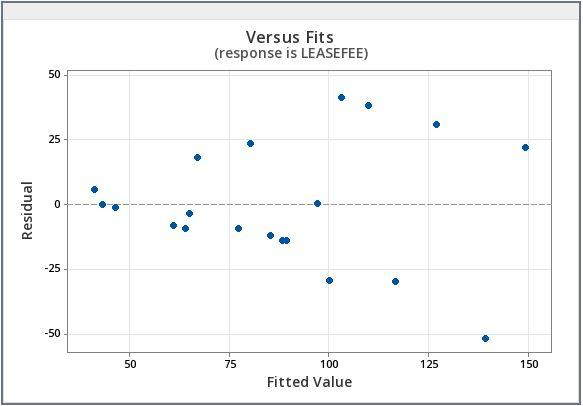
\includegraphics[width=0.8\textwidth]{Residual_vs_Fitted.jpeg}
    \caption{residual vs. fitted}
\end{figure}







\end{document}